\documentclass[a4paper,12pt, twoside]{article}
%\documentclass[a4paper,12pt, twoside]{book}

\usepackage[papersize={210mm,297mm},tmargin=20mm,bmargin=20mm,lmargin=20mm,rmargin=20mm]{geometry}

\usepackage[utf8]{inputenc}
%https://mirror.hmc.edu/ctan/macros/latex/contrib/babel-contrib/turkish/turkish.pdf
\usepackage[turkish, english]{babel}
%\usepackage[T1]{fontenc}

\usepackage{amsmath,amssymb,mathabx}%\for eqref
\usepackage{lscape}

%%% \usepackage{svg}
%%% https://tex.stackexchange.com/questions/122871/include-svg-images-with-the-svg-package/129854
\usepackage{graphicx}
\graphicspath{ {./figurler/} }

\usepackage[colorinlistoftodos]{todonotes}
\usepackage{fancyhdr}

\usepackage{indentfirst}
%% paragraf girintisi
\setlength{\parindent}{5ex}

\pagestyle{fancy}
\fancyhf{}
\lhead{ Kuantum Fiziği }
\chead{\thepage}
\rhead{Mesut Karakoç}
\lfoot{Akdeniz Üniversitesi}
\cfoot{}
%\rfoot{BF}

\title{Akdeniz Üniversitesi\\ Fen Fakültesi - Fizik Bölümü\\FİZ319 Kuantum Fiziği Ders Notları}

\author{\setlength{\unitlength}{6mm}
\begin{picture}(10,10)
\put(1.1,0){\includegraphics[width=4.5cm]{Leptonic_event_in_Gargamelle_bubble_chamber.jpg}}
\end{picture} \\ Doç. Dr. Mesut Karakoç}


\date{\today}

\begin{document}

%% Turkish babel problem
%% https://tex.stackexchange.com/questions/160385/newgeometry-doesnt-work-with-turkish-babel-package
\shorthandoff{=}% Make = not active any more

\maketitle

\newpage

\renewcommand{\contentsname}{İçindekiler}
\tableofcontents{İçindekiler}

\newpage

{
\hspace{.5\textwidth}
\begin{minipage}{.5\textwidth}
\raggedleft
For, as it has once been said, ``research is to see what everybody has seen and to think what nobody has thought." But post iacturam quis non sapit! \cite{book:Jammer}



%% Latince için
%% post iacturam quis non sapit!
%% Who is not wise after he has lost something?
%% https://quizlet.com/23756827/latin-proverbs-h-flash-cards/
\end{minipage}
}


\section{Kuantum Fiziğinin Ortaya Çıkışı}

Kuantum fiziğinin doğum sürecinin 14 Aralık 1900 tarihinde başladığı kabul edilebilir. O gün Max Planck Alman Fizik Topluluğu'nun bir toplantısında ``Normal Spektrumun Enerji Dağılım Yasasının Teoremi" başlıklı makalesini sunmuştu \cite{book:EisbergResnick}. Bu makale çok ilgi görmemesine rağmen, bir elektronun enerjisinin kuantumlu olabileceğini ilk defa öne sürdüğü için önemlidir.

Kuantum fiziğinin bütünüyle sadece bu makaleyle başladığını söylemek pek doğru olmaz. On dokuzuncu yüzyılın başlarında gerçekleştirilen bazı deneyleri klasik fizik açıklamakta yetersiz kalmıştır. Bu ilk bölümde bu deneyleri ve bu deneylerin açıklanması için ortaya çıkan yeni kavramları (ışığın parçacık özelliği, maddenin dalga davranışı, fiziksel niceliklerin kuantumlanması) anlamaya çalışacağız. 


\subsection{Karacisim Işıması}

% Modern Physics
% Michael Fowler, University of Virginia
% http://galileo.phys.virginia.edu/classes/252/black_body_radiation.html
% Black Body Radiation
% http://galileo.phys.virginia.edu/classes/252/


\subsubsection{Klasik Fiziğe Göre}
On dokuzuncu yüzyılın başlarında fizikçilerin en çok ilgilendikleri konulardan birisi:
ısıtılmış cisimlerin nasıl ışıma yaptıklarıdır? Bu nedenle ısıtılmış cisimlerin ışıması üzerine bir çok deney yapılmış ve teorik olarak açıklanmaya ihtiyaç duyan bir çok deneysel veri ortaya çıkmıştır \cite{book:Sharkov}. Termal ışımalar üzerine teorik çalışmalar Gustav Kirchhoff'un 1859 yılındaki çalışmaları ile başlar \cite{book:Gasiorowicz}. 

Kirchhoff ``Işık ve ısının yayılımı ve soğurulması arasındaki ilişki" \cite{book:Jammer, Kirchhoff1859} adlı makalesinde etrafları mükemmel yansıtıcılarla sarılmış iki yayıcı ve soğurucu sonsuz paralel plakanın ısıl denge durumundaki ışınım alış verişlerini inceledi. Plakaların yayıcılık (Emitting) ve soğuruculuk (Absorbing) özelikleri için $E(\lambda, T)$ ve $A(\lambda, T)$ şeklinde iki ifade tanımladı. 

\begin{itemize}
\item $E(\lambda, T)$: yayınlanma gücü herhangi bir $T$ sıcaklığında  herhangi bir $\lambda$ dalga boyundaki ışımanın birim alan ve birim zaman başına şiddetini tanımlar ve birimi $W/m^2\equiv \frac{J}{s} \frac{1}{m^2}$'dir.
\item $E/A$ yayınlanan ışının ne kadarlık kısmının soğurulduğunu tanımlar.
\end{itemize}

Kirchhoff ortaya attığı problemdeki termal denge durumundaki levhalardan birinden yayınlanan ışınımın enerjisinin diğeri tarafından soğurulanın enerjisine eşit olması gerektiğini gösterdi ve böylece her iki plaka içinde $E/A$ oranının eşit olacağını gösterdi.

Daha sonra Kirchhoff ``kara cisim" diye adlandırdığı bütün ışık spektrumunu soğurabilen bir nesne kavramını ortaya attı ve bu nesne için $A=1$ olduğunu fark etti. Bu durumda $E(\lambda, T)$ bütün termal ışıma yapan nesneler için evrensel bir fonksiyon halini almaktadır.


%\shorthandoff{=}% Make = not active any more
\begin{figure}
\center
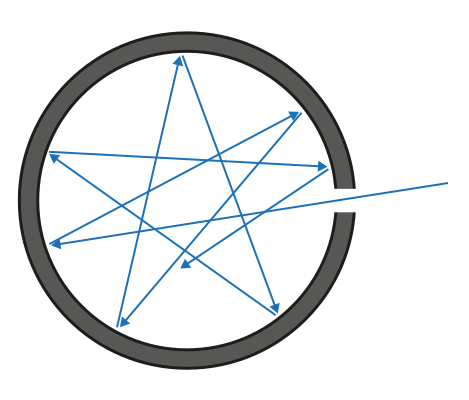
\includegraphics[scale=.5]{Black_body_realization.pdf}
\caption{Kara cisim, küre şeklindeki kovukta açılan deliktir.}
\label{fig:karacisim}
\end{figure}
%\shorthandon{=}% Make = active again

Böyle bir karacisim şekilde gibi bir küresel kovukta açılan delikle temsil edilir. Bu deliğe gelen neredeyse bütün elektromanyetik ışınlar tekrar kovuktan çıkamazlar ve kovuk duvarları tarafından soğurulurlar. Böylece kovuğun bu çok küçük deliği bütün elektromanyetik spektrumu soğuran bir kara cisim halini alır.

\begin{itemize}
\item Termodinamiğin ikinci yasısına göre yalıtılmış bir sistemin entropisi ya artar ya da ideal bir denge durumunda sabit kalır.
\end{itemize}

%% Termodinamik yasalar:
%% The zeroth law of thermodynamics states that if two thermodynamic systems each are in thermal equilibrium with a third, then they are in thermal equilibrium with each other. Accordingly, thermal equilibrium between systems is a transitive relation.

%% The first law is often formulated[1][nb 1] {\displaystyle \Delta U=Q-W.} {\displaystyle \Delta U=Q-W.} It states that the change in the internal energy ΔU of a closed system is equal to the amount of heat Q supplied to the system, minus the amount of work W done by the system on its surroundings. An equivalent statement is that perpetual motion machines of the first kind are impossible.

%% The second law of thermodynamics states that the total entropy of an isolated system can never decrease over time. The total entropy can remain constant in ideal cases where the system is in a steady state (equilibrium), or is undergoing a reversible process. In all spontaneous processes,[1] the total entropy increases and the process is irreversible. The increase in entropy accounts for the irreversibility of natural processes, and the asymmetry between future and past.[2]

%% The third law of thermodynamics is sometimes stated as follows, regarding the properties of closed systems in thermodynamic equilibrium: The entropy of a system approaches a constant value as its temperature approaches absolute zero.

Kirchhoff bu yasaya dayanarak kovuğun içinde termal ışımanın homojen olması gerektiğini ve ışıma akısının yönden bağımsız olması gerektiğini ve aynı sıcaklığa sahip herhangi bir kovuk sistemi için bu durumun geçerli olduğunu gösterdi.

Kovuğun içindeki enerji yoğunluğunun ($w(\lambda,T)$) yayınlama gücü $E$ ile olan ilişkisi aşağıdaki gibidir,
 
\begin{equation}
\label{eq:emissiveDensity}
w(\lambda,T) = \frac{4 E(\lambda,T)}{c}.
\end{equation}
%%
burada $c$ ışığın boşluktaki hızıdır. Wilhelm Wien 1894 yılında enerji yoğunluğunun (deneysel verilerin bir sonucu olarak), 
%%
\begin{equation}
\label{eq:f_lambdaT}
w(\lambda,T) = \lambda^{-5} f(\lambda T)
\end{equation}
%%
%%
\begin{figure}[hbtp]
\center
\includegraphics[scale=.4]{blackbody_spect_vs_lambdaT.png}
\caption{Denk. \ref{eq:f_lambdaT}'deki fonksiyonun varlığını gösteren spektrum.}
\label{fig:karaSpektrum_lamdaT}
\end{figure}
%%
gibi bir fonksiyon cinsinden yazılabileceğini gösterdi. Bu fonksiyonun bir benzerini frekansa bağlı olarak aşağıdaki eşitliği kullanarak yazmak da mümkündür.

\begin{equation}
\label{eq:uw_densities}
u(\nu,T) = w(\lambda,T)\left|\frac{d\lambda}{\nu}\right| = w(\frac{c}{\nu},T)\frac{c}{\nu^2}.
\end{equation}
%%
Böylece Wien'in önerdiği tek parametreli bilinmeyen fonksiyon,
%%
\begin{equation}
\label{eq:ug_lambdaT}
u(\nu,T) = \nu^3 g(\frac{\nu}{T})
\end{equation}
%%
olarak da önerilebilir. Wien bilinmeyen bu fonksiyon için Lummer ve Pringsheim tarafından önerilen deneylere dayanarak,
%%
\begin{equation}
\label{eq:g_lambdaT}
g(\nu/T) = C e^{-\beta \nu/T}
\end{equation}
%%
formunu önermiştir ve ışıma spektrumun yüksek frekanslı (düşük dalga boylu) kısımlarını açıklamayı başarmıştır. Yine aynı fonksiyondan faydalanarak,
%%
\begin{equation}
\label{eq:wien_shift}
\lambda_{enb} = b/T 
\end{equation}
%%
%%
\begin{figure}[hbtp]
\center
\includegraphics[scale=.4]{blackbody_spect_vs_wavelength.png}
\caption{3000, 4000 ve 5000 Kelvin sıcaklıklarındaki sistemlerin kara cisim spektrumları.}
\label{fig:karaSpektrum}
\end{figure}
%%
%%
Wien kayma yasası olarak bilinen eşitliği bulmuştur. Burada $b = 2.8977729(17)\times10^{-3}$ m K değerindedir ve biraz önce bahsedilen deneyden elde edilen bir sabittir. Bütün kara cisim spektrumları için geçerlidir. Bu yasa ile belirli bir sıcaklıkta hangi dalga boyunda en büyük ışıma şiddetinin gerçekleşeceği belirlenebilir.

Örneğin Şekil \ref{fig:karaSpektrum}'teki spektrumlar için Wien yasasından faydalanılarak Tablo \ref{tab:wien_shift}'deki değerler bulunur.
%%
%%
\begin{table}[hbtp]
\center
\begin{tabular}{|c|c|}
\hline
T ($^\circ$K) & $\lambda_{enb}\,(\mu m)$\\
\hline
3000 & 0.966 \\
4000 & 0.724 \\
5000 & 0.580 \\
\hline
\end{tabular}
\caption{\label{tab:wien_shift} Wien kayma yasası ile elde edilen dalga boyu değerleri. Şekil \ref{fig:karaSpektrum}'de spektrum eğrileri üzerinde içi dolu noktalar olarak işaretlenmişlerdir.}
\end{table}
%%

Wien'in modeli yüksek frekanslarda deneyle uyumlu olmasına karşın düşük frekanslarda bu başarıyı yakalayamamıştır. Ek olarak Wien'in modeli klasik fiziğin temel bazı varsayımlarını göz önüne almamamıştır. J. W. S. Rayleigh klasik fizikteki enerjinin eş bölüşümü teoremini ve elektromanyetik dalgaların kovuk içerisindeki normal modlarını hesaba katarak,
%%
% eş bölüşüm teoremi
% https://en.wikipedia.org/wiki/Equipartition_theorem#cite_note-4
%
\begin{equation}
\label{eq:Rayleigh}
u(\nu, T) = \frac{8 \pi \nu^{2}}{c^{3}} k_{B} T
\end{equation}
sonucuna ulaşmıştır. Burada $k_B = 1.38064852 \times 10^{-23}$ J/K, Boltzmann sabitidir ve enerjinin eş bölüşüm teoremine göre $k_B T$ serbestlik derecesi başına ortalama enerjidir. Elde edilen bu dağılım Rayleigh-Jeans dağılımı olarak bilinir. Jeans'in katkısı Rayleigh'in hesaplarında yaptığı bir düzeltmeden kaynaklanmaktadır. Rayleigh-Jeans dağılımı Wien dağılımının aksine yüksek frekanslarda başarısızdır. Ek olarak bütün frekanslar üzerinden alınan integral sonucunda elde edilen kovuk içindeki toplam enerji yoğunluğu ıraksar ve sonsuz değer verir, böylece fiziksel açıdan doğru olmayan bir sonuç elde edilmiş olur.






\subsubsection{Planck Dağılımı ve Kuantumlu Enerji Kavramı}

Planck, Wien ve Rayleigh-Jeans dağılımlarını dikkate alarak deneysel eğriyi çok iyi açıklayan,
%%
\begin{equation}
\label{eq:Planck}
u(\nu, T) = \frac{8 \pi h}{c^{3}} \frac{\nu^{3}}{e^{\frac{h \nu}{k_{B} T}} - 1}
\end{equation} 
%%
dağılım formülünü elde etmiştir. Burada $h$ daha sonra çok ünlenen fakat Planck tarafından sadece deneysel ve teorik eğriyi birbirine uydurabilmek için eklenmiş bir serbest parametredir. Serbest parametrenin(!) değerinin $h=6.626070040 \times 10^{-34}$~J~s olduğu bulunmuş ve adına Planck sabiti denmiştir.Planck'ın elde ettiği dağılım ifadesi $\frac{h\nu}{k_B T}<<1$ için Rayleigh-Jeans dağılımına indirgenirken, $\frac{h\nu}{k_B T}>>1$ için Wien dağılımana indirgenmektedir.

\begin{figure}[hbtp]
\begin{minipage}{0.49\textwidth}
\center
\includegraphics[scale=.22]{blackbody_spect_vs_frequency_diff_models.png}
\caption{Üç farklı modelle elde edilen kara cisim ışıma spektrumlarının frekansa göre davranışı.}
\label{fig:karaSpektrum_nu}
\end{minipage}
\hspace{12pt}
\begin{minipage}{0.49\textwidth}
\center
\includegraphics[scale=.22]{blackbody_spect_vs_wavelength_diff_models.png}
\caption{Üç farklı modelle elde edilen kara cisim ışıma spektrumlarının dalga boyuna göre davranışı.}
\label{fig:karaSpektrum_lambda}
\end{minipage}
\end{figure}

Planck ilk önceleri bu ifade için teorik bir temel kuramasa da daha sonra, kovuğun duvarlarındaki ışınımın yayılma ve soğurulma dinamik dengesini izah edebilmek için kovuğun duvarlarının basit salınıcılar (osilatör) gibi davrandığını ortaya atmıştır. Bu düşünceyi ortaya atarken önemli bir varsayımda bulunmuştur: ``herhangi bir  $\nu$ frekanslı ışınımın sadece $\large \boldsymbol{E=h\nu}$ enerjili paketler (kuanta) halinde yayılabilir veya soğurabilir".

Boltzmann dağılımı ile kara cisim kovuğu içindeki ortalama enerji,
%%
\begin{equation}
\label{eq:AvE_Boltzmann}
\overline E =\frac{\int \limits_0^\infty E P(E) dE}{\int \limits_0^\infty P(E) dE} 
\end{equation} 
%%
ifadesi ile hesaplanabilir. Burada $P(E)$ basit harmonik salınıcıların $E$ enerjisine sahip olma olasılığını tanımlayan Boltzmann dağılımıdır ve
%%
\begin{equation}
\label{eq:Boltzmann}
P(E) = \frac{e^{-E/k_BT}}{k_BT}
\end{equation} 
%%
olarak tanımlanır. Planck $E$'nin sürekli bir değişken değilde izinli ve kesik değerlere sahip olmasını gerektiğini düşündüğünden, $n = 0, 1, 2, \dots$  olmak üzere, Denk. \ref{eq:AvE_Boltzmann},
%%
\begin{equation}
\label{eq:Boltzmann_Planck}
\overline E =\frac{\sum \limits_{n=0}^\infty E P(E)}{\sum \limits_{n=0}^\infty P(E)} 
\end{equation}
%%
olarak yazılabilir. Böylece, herhangi bir radyasyon yayılımı ve soğurulması $E=nh\nu$ enerjili değerler alabildiğine göre,
%%
\begin{equation}
\label{eq:Boltzmann_Planck}
\overline E =\frac{\sum \limits_{n=0}^\infty nh\nu \frac{e^{-E/k_BT}}{k_BT}}{\sum \limits_{n=0}^\infty \frac{e^{-E/k_BT}}{k_BT}} 
\end{equation}
%%
sonucuna ulaşılır. Gerekli matematiksel işlemler tamamlandığında \cite{book:EisbergResnick} kovuk içi basit salınıcıların (harmonik osilatörlerin) ortalama enerjisi,
%%
\begin{equation}
\label{eq:Planck_Av_E}
\overline E = \frac{h\nu}{e^{\frac{h \nu}{k_{B} T}} - 1}
\end{equation}
%%
olarak bulunur. Elde edilen bu sonuç birim hacimdeki harmonik osilatör sayısı ile çarpıldığında Denk. \ref{eq:Planck}'deki Planck dağılımı elde edilmiş olur. 

Şekil \ref{fig:karaSpektrum_nu} ve \ref{fig:karaSpektrum_lambda}'te sürekli çizgiyle çizilen dağılım Planck dağılımıdır ve deneysel verileri en iyi açıklayan dağılımdır. Ek olarak Planck enerji yoğunluğu dağılımının bütün frekanslar üzerinden integrali alındığında Rayleigh-Jeans gibi ıraksamaz ve sonlu bir değerde kalır. Integral ve sonucu aşağıdaki gibidir.
%%
\begin{equation}
\label{eq:Planck_U_total}
U(T) = \frac{8 \pi h}{c^{3}} \int\limits_0^\infty d\nu \frac{\nu^{3}}{e^{\frac{h \nu}{k_{B} T}} - 1} = a T^4
\end{equation}
%%
Eğer integral yayınım gücü yoğunluğu üzerinden alınmış olsaydı sonuç,
%%
\begin{equation}
\label{eq:Planck_E_total}
E(T) = \sigma T^4
\end{equation}
%%
olurdu. Her iki ifade de karacisim ışınımı için benzeri bir sonucu ifade etmektedir ve Stefan-Bolzman yasası olarak bilinmektedir: ``bütün ışıma spektrumu üzerinden alınan integral sonucu elde edilen ışıma enerji yoğunluğu veya ışıma yayınım gücü sıcaklığın dördüncü kuvvetiyle doğru orantılıdır". Her iki ifadedeki sabitlerin değerleri,
%%
\begin{eqnarray}
\label{eq:stefan_boltzman}
\sigma &=&  5.670367(13) \, \times 10^{-8}\ \textrm{W}\,\textrm{m}^{-2}\,\textrm{K}^{-4} \\
a &=& 4\frac{\sigma}{c} \nonumber
\end{eqnarray}
%%
olarak verilir ve $\sigma$ Stefan-Boltzmann sabiti \cite{codata:stefan_boltzman} olarak adlandırılır.


Planck neden bu şekilde kesikli bir davranışın gerçekleştiğine bir açıklama getiremedi ve bilinmeyen bir neden kovuk duvarlarındaki atomların paketler (kuantlar) halinde kesikli enerjiler yayınladıklarını öne sürdü. Bilinmeyen nedenin açıklaması fotoelektrik etkinin Einstein tarafından çalışılmasıyla ortaya çıktı.

Günlük hayatımızda ışığın kesikli veya parçacıklı doğasını görememiz doğaldır. Örneğin, beyaz ışık yayan ve 5 Watt'lık tasarruflu bir ampulden gözümüze 400 nm (mor) ve 700 nm (kırmızı) dalga boyu aralığında bir çok ışık gelmektedir. Ampülden gelen bütün ışığın en küçük dalga boyuna yani en fazla enerjiye sahip olduğunu varsayalım. Bu durumda bir tek ışık paketinin sahip olacağı enerji,
%%
\begin{equation}
\label{eq:example_light_quanta01}
h\nu = h c/\lambda = \frac{6.63\times10^{-34}\,\,3\times10^{8}}{400\times10^{-9}} \eqsim 5\times 10^{-19} J 
\end{equation}
%%
olur. Bu çok küçük bir enerji miktarıdır. 5 Watt'lık tasarruflu ampülün bir saniyede yayınlayacağı ışık paketi sayısı ise,
%%
\begin{equation}
\label{eq:example_light_quanta02}
N = \frac{5\,J/s}{5\times10^{-19}\,J} \eqsim 10^{19} paket/s
\end{equation}
%%
olur.Bu miktarda paketin bir saniyede insan tarafından tek tek sayılması mümkün değildir!

% CMB: Cosmic Microwave Background
% https://wmap.gsfc.nasa.gov/universe/bb_cosmo_fluct.html
% https://en.wikipedia.org/wiki/Chronology_of_the_universe
% https://simple.wikipedia.org/wiki/Cosmic_microwave_background_radiation

% YOUTUBE
% https://www.youtube.com/watch?v=LnmCsNQsR68
% https://www.youtube.com/watch?v=HnBZf1RfB-w



\subsection{Fotoelektrik Etki}

1860'larda Maxwell ünlü Elektrik ve Manyetik alan denklemlerini yazdı, bu denklemer elektrik yükünün olmadığı bir yerde 
%%
\begin{align}
\label{eq:maxwell}
  \vec \nabla \cdot \vec{E} &= 0 \quad & \nabla \times \vec{E} &=              -\frac{\partial\vec B}{\partial t}, \\
    \vec \nabla \cdot \vec{B} &= 0 \quad & \nabla \times \vec{B} &= \mu_0\varepsilon_0 \frac{\partial\vec E}{\partial t}.
\end{align}
%%
şeklini alırlar. Bu denklemlerden faydalanarak Elektrik ve Manyetik alanının zamanla davranışını Elektromanyetik (EM) dalga olarak aşağıdaki denklemlerle tanımladı. 
%%
\begin{align}
\label{eq:maxwell_EM_wave}
  \mu_0\varepsilon_0  \frac{\partial^2   \vec{E}}{\partial t^2} - \nabla^2   \vec{E} = 0 \\
  \mu_0\varepsilon_0 \frac{\partial^2   \vec{B}}{\partial t^2} - \nabla^2 \vec{B} = 0
\end{align}
%%
Işığın da bu denklemlere uygun davranış gösteren EM dalgaları olduğu biliniyordu. Denk. \ref{eq:maxwell_EM_wave} dalga denklemlerinin çözümüyle belirlenen bu EM dalgaları boşlukta, 
%%
\begin{align}
\label{eq:EM_waves}
\vec E = \vec E_0 \sin(kz-\omega t),\hspace{36pt} \vec B = \vec B_0 \sin(kz-\omega t), 
\end{align}
%%
ifadeleri ile tanımlanırlar. Burada $k=2\pi\lambda$ dalga sayısı ve $\omega=2\pi\nu$ açısal frekanstır. EM dalgaları temsili olarak aşağıdaki şekildeki gibi ilerler ve enerji taşırlar.
%%
\begin{figure}[hbtp]
\center
\includegraphics[scale=1.2]{EM_wave_poynting_vector.png}
\caption{$+z$ yönünde ilerleyen düzlem EM dalgalar.}
\label{fig:poynting}
\end{figure}
%%
EM dalgalarının taşıdığı enerjinin akısı matematiksel olarak ise Poynting vektörü ile tanımlanır. Yukarıdaki düzlem dalgalar için,
%%
\begin{align}
\label{eq:poynting_vec}
\vec S = \frac{1}{\mu_0}\vec E \times \vec B
\end{align}
%%
genel tanımından yola çıkarak,
%%
\begin{align}
\label{eq:poynting_plane_wave}
\vec S = \frac{1}{\mu_0} E_0 B_0 \sin^2(kz-\omega t)\hat z
\end{align}
%%
olarak bulunur. Poything vektörü birim alan başına aktarılan gücü ($W/m^2$) veya birim alan başına birim zamanda aktarılan enerjiyi ($J/s/m^2$) tanımlar. Eğer $x-y$ düzlemine paralel $z$ eksenine dik $A$ alanına sahip bir dedektör yüzeyine aktarılacak gücü hesaplamak istersek,
%%
\begin{align}
\label{eq:poynting_power1}
P = S A
\end{align}
%%
ile hesaplayabiliriz. EM dalgasının elektrik ve manyetik alan bileşenlerinin genlikleri arasında $B_0 = E_0/c$ bağıntısı olduğunu da hatırlayarak,
%%
\begin{align}
\label{eq:poynting_power2}
P = \frac{1}{\mu_0 c} E_0^2 A \sin^2(kz-\omega t)
\end{align}
%%
ile dedektöre aktarılan gücü hesaplayabiliriz. Böylece klasik olarak ışığın bir yüzeye aktarabileceği gücün (veya şiddetin $I = P/A$) elektrik veya manyetik alanın genliğinin karesiyle orantılı olduğu görülür.

Fakat, 1887'de Heinrich Hertz tarafından gerçekleştirilen fotoelektrik etki deneyi ışığın EM dalga davranışına aykırı sonuçlar ortaya koydu.
%%
\begin{figure}[hbtp]
\center
\includegraphics[scale=.5]{fotoeletrik_deney_devresi.png}
\caption{Hertz tarafından kullanılan deney düzeneğinin şeması \cite{book:EisbergResnick}.}
\label{fig:fotoeletrik_devresi}
\end{figure}
%%
Deneyde basitçe, A metal plakasına gelen tek renkli ışık eğer elektron koparabilirse ve bu koparılan elektron B plakasına ulaşabilirse $G$ ampermetresinde bir akım okunmaktadır. Böyle bir deney düzeneğinden klasik EM teoremine göre elektronların koparılabileceği ve dolayısıyla fotoelektrik etkinin izah edileceği düşünülebilir. Buna göre klasik fiziğin fotoelektrik etki için tahminleri \cite{book:KraneS} aşağıdaki gibi özetlenebilir.
\begin{itemize}
\item {\bf Koparılan elektronların sahip olabileceği en büyük kintetik enerji ışığın şiddetiyle orantılı olmalıdır:} Işığın şiddeti arttıkça $E$ artmalı, $E$ arttıkça $I=P/A$ artmalıdır. Böylece bir elektrona aktarılan enerji artmalıdır.

\item {\bf Fotoelektrik etki ışığın frekansından veya dalga boyundan bağımsızdır:} Işığın şiddeti yeterliyse frekansı ne olursa olsun elektron koparılabilmelidir.

\item {\bf Işık $A$ plakasına vardıktan sonra saniye mertebesindeki sürelerde plakadan elektron yayınlanır:} $\Delta E/\Delta t = P_{ort}$ ifadesinden bir elektronu koparmak için ne kadar süre harcanması gerektiği hesaplanabilir. Burada $\Delta E$ elektron koparmak için gerekli enerji, $P_{ort}$ gönderilen ışığın ortalama gücü ve $\Delta t$ elektronun koparılma süresidir.
\end{itemize}



\subsection{Compton Etkisi}

% In the preamble, add "\renewcommand\refname{New Title}" for article type documents 
% and "\renewcommand\bibname{New Title}" for book and report type documents.
\renewcommand\refname{Kaynaklar}
\bibliography{quantumBIB}{}
%% https://www.sharelatex.com/learn/latex/bibtex_bibliography_styles
 \bibliographystyle{plain}
%% \bibliographystyle{alpha}
%%\bibliographystyle{apalike}
\end{document}

